La technique est similaire au cas du triangle: nous allons obtenir une condition nécessaire, puis nous verrons que cette condition suffit via des arguments d'analyse. Cette dernière section nécessite plus de technicité.


% ----------------------- %


\begin{defi}
	Un \og \emph{\ngone} \fg\ désigne un polygone à $n$ côtés de mesure non nulle, avec $n \geq 3$.
\end{defi}


\begin{defi}
	Un \og \emph{\niso} \fg\ désigne un \ngone\ dont tous les côtés sont de mesure égale.
\end{defi}


% ----------------------- %


\begin{fact} \label{conv-poly}
	Si un \ngone\ $\setproba{P}$ n'est pas convexe, alors on peut construire un \ngone\ convexe $\setproba{P}^{\,\prime}$ tel que 
	$\perim{\setproba{P}^{\,\prime}} = \perim{\setproba{P}}$ 
	et 
	$\area{\setproba{P}^{\,\prime}} > \area{\setproba{P}}$.
\end{fact}


\begin{proof}
	Ici, il ne faut pas être expéditif en indiquant que la preuve du fait \ref{quadri} se généralise sans aucun souci.
	En effet, avec $n > 4$, nous pouvons avoir plusieurs points de non-convexité, et les éliminer comme nous l'avons fait pour le quadrilatère n'est pas immédiat:
	dans la figure suivante, l'élimination des deux points de non convexité $G$ et $E$ de l'heptagone $ABCDEFG$ nous amène à un nouvel heptagone $ABCDE^{\,\prime}FG^{\,\prime}$ ayant lui aussi deux points de non-convexité $F$ et $D$!
	Donc, rien n'empêche, a priori, d'avoir une suite de constructions n'aboutissant jamais à un heptagone convexe
	de même périmètre que celui de $ABCDEFG$, et d'aire strictement supérieure à celle de $ABCDEFG$.%
	\footnote{
		L'auteur est convaincu que le procédé aboutira en un nombre fini d'étapes à un polygone convexe, mais il ne l'a pas démontré pour le moment.
	}

	\begin{center}
		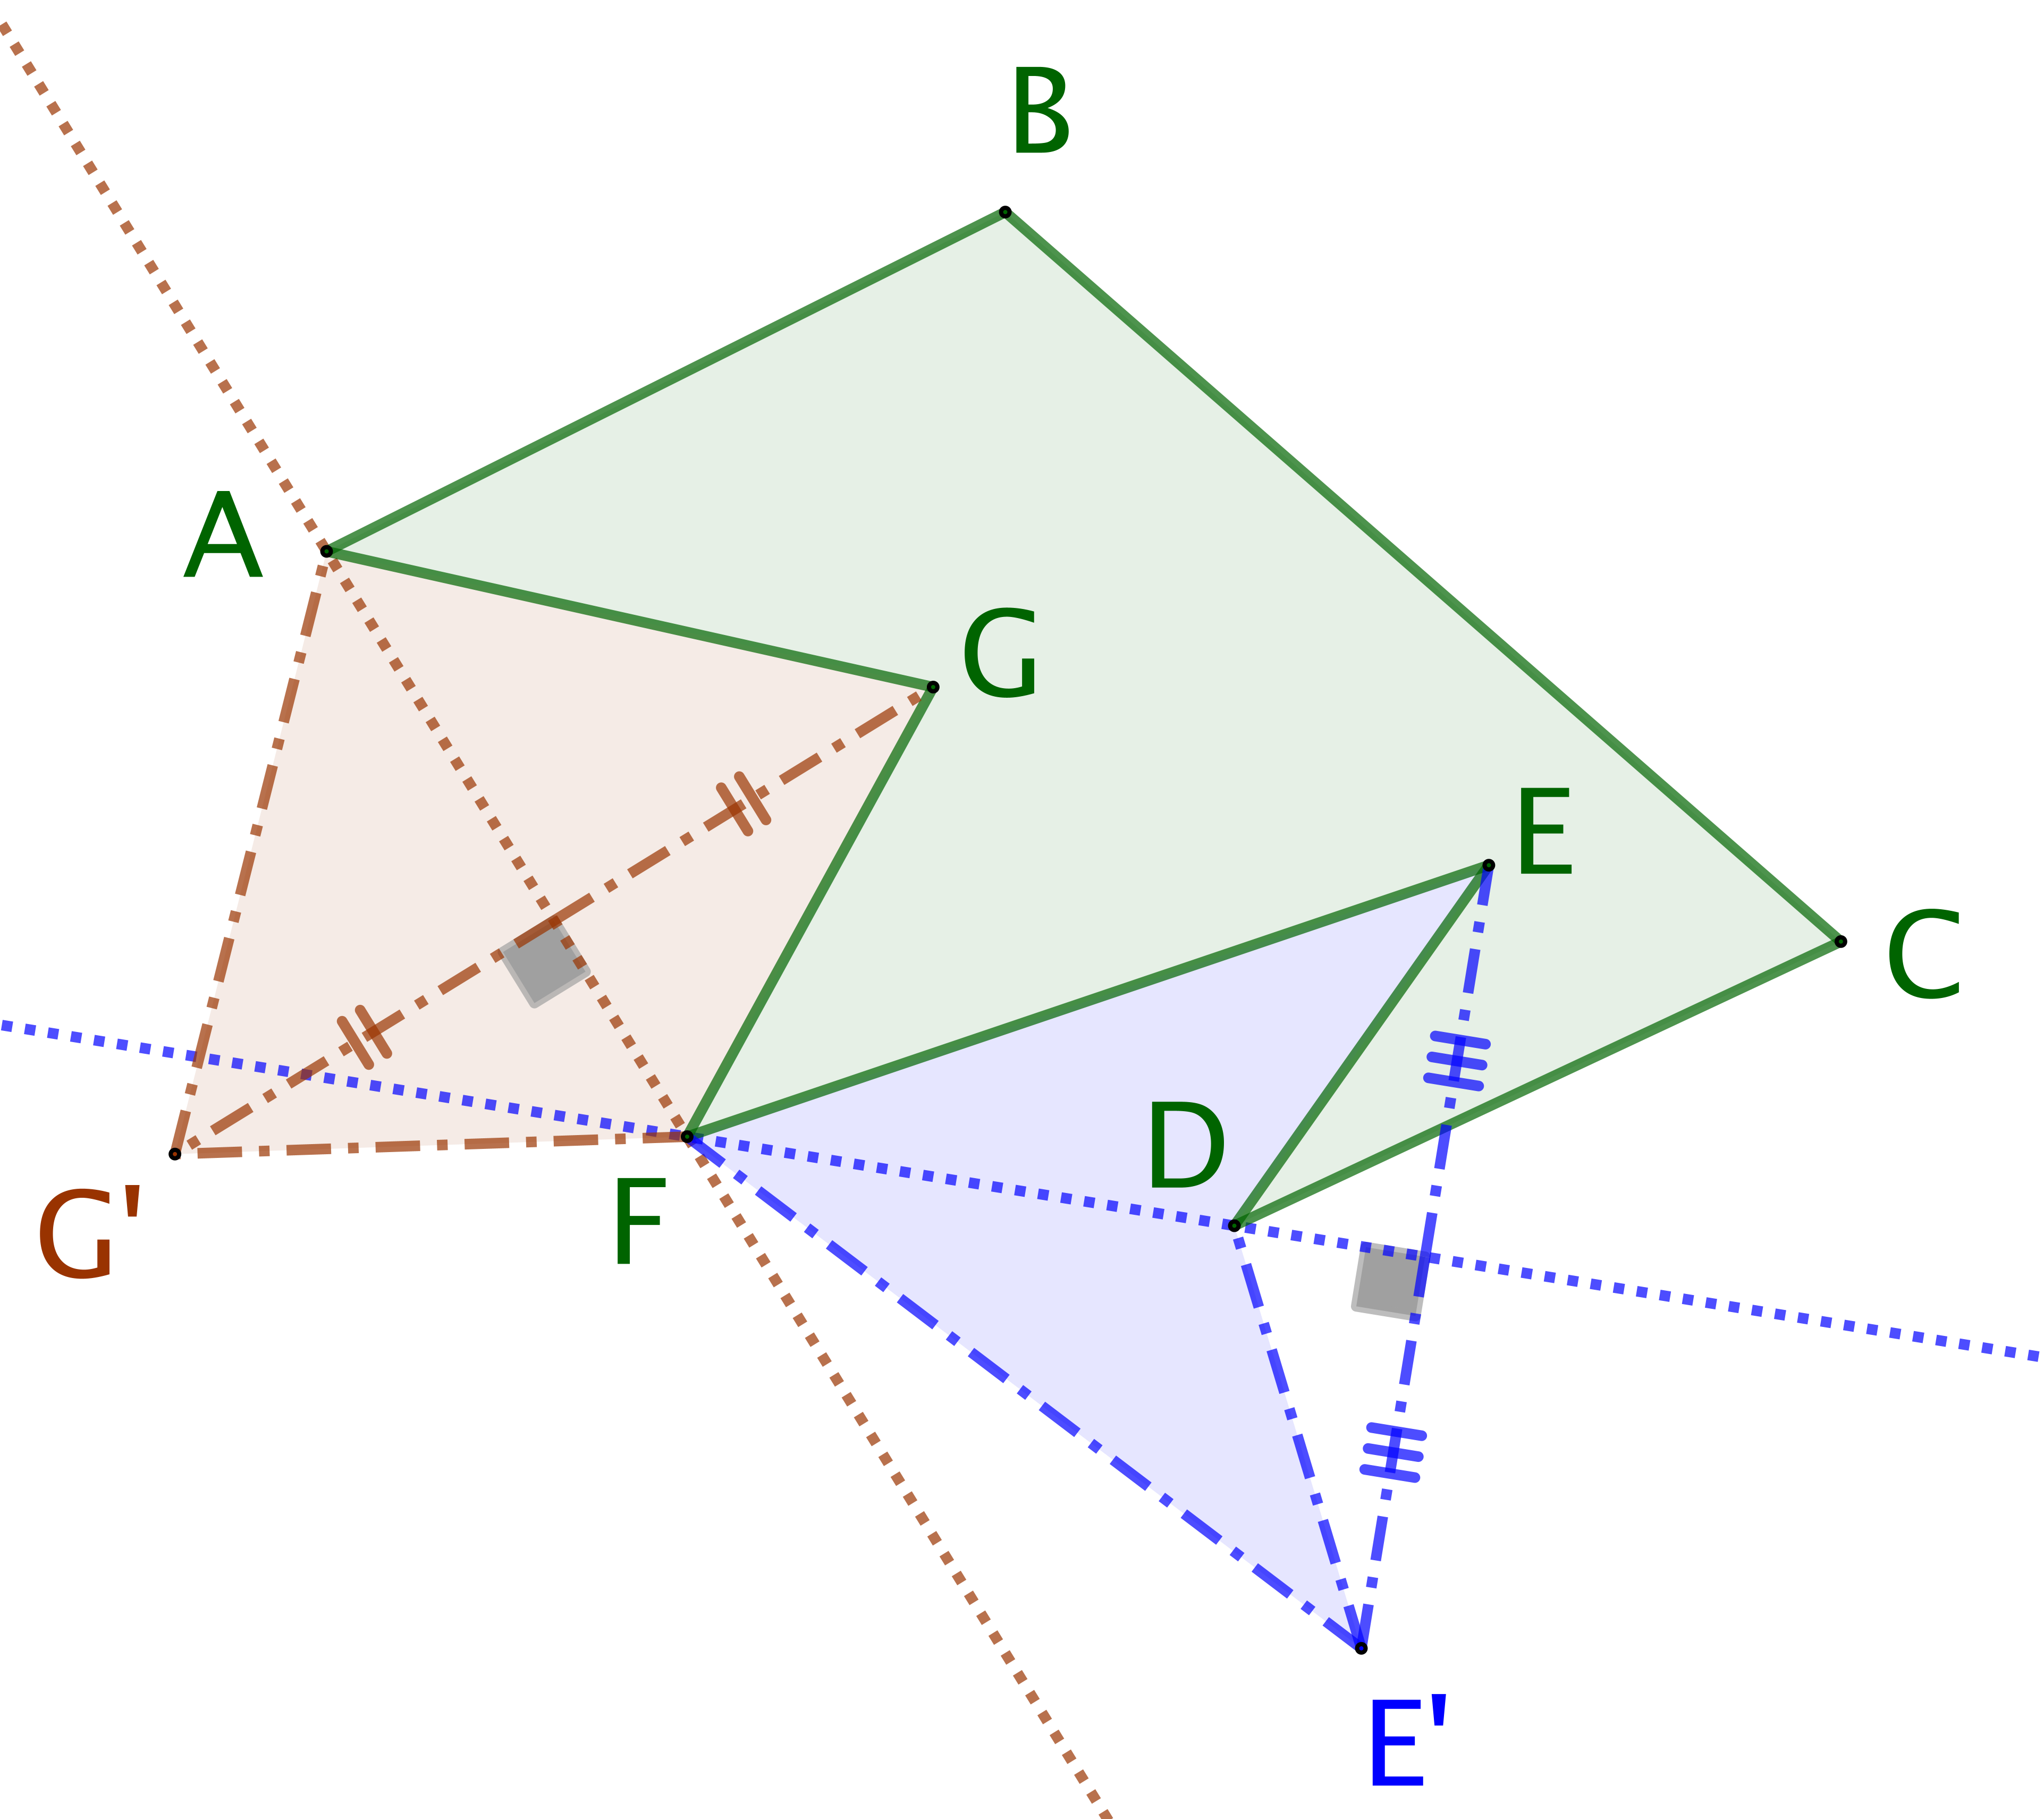
\includegraphics[scale=.4]{content/polygon/polygon-non-convex-trap.png}
	\end{center}
	

	On peut aussi perdre des côtés lors de la construction comme dans l'exemple suivant où $C$, $D$ et $E^{\,\prime}$ sont alignés. Nous allons voir juste après que ce problème n'en est pas un.

	\begin{center}
		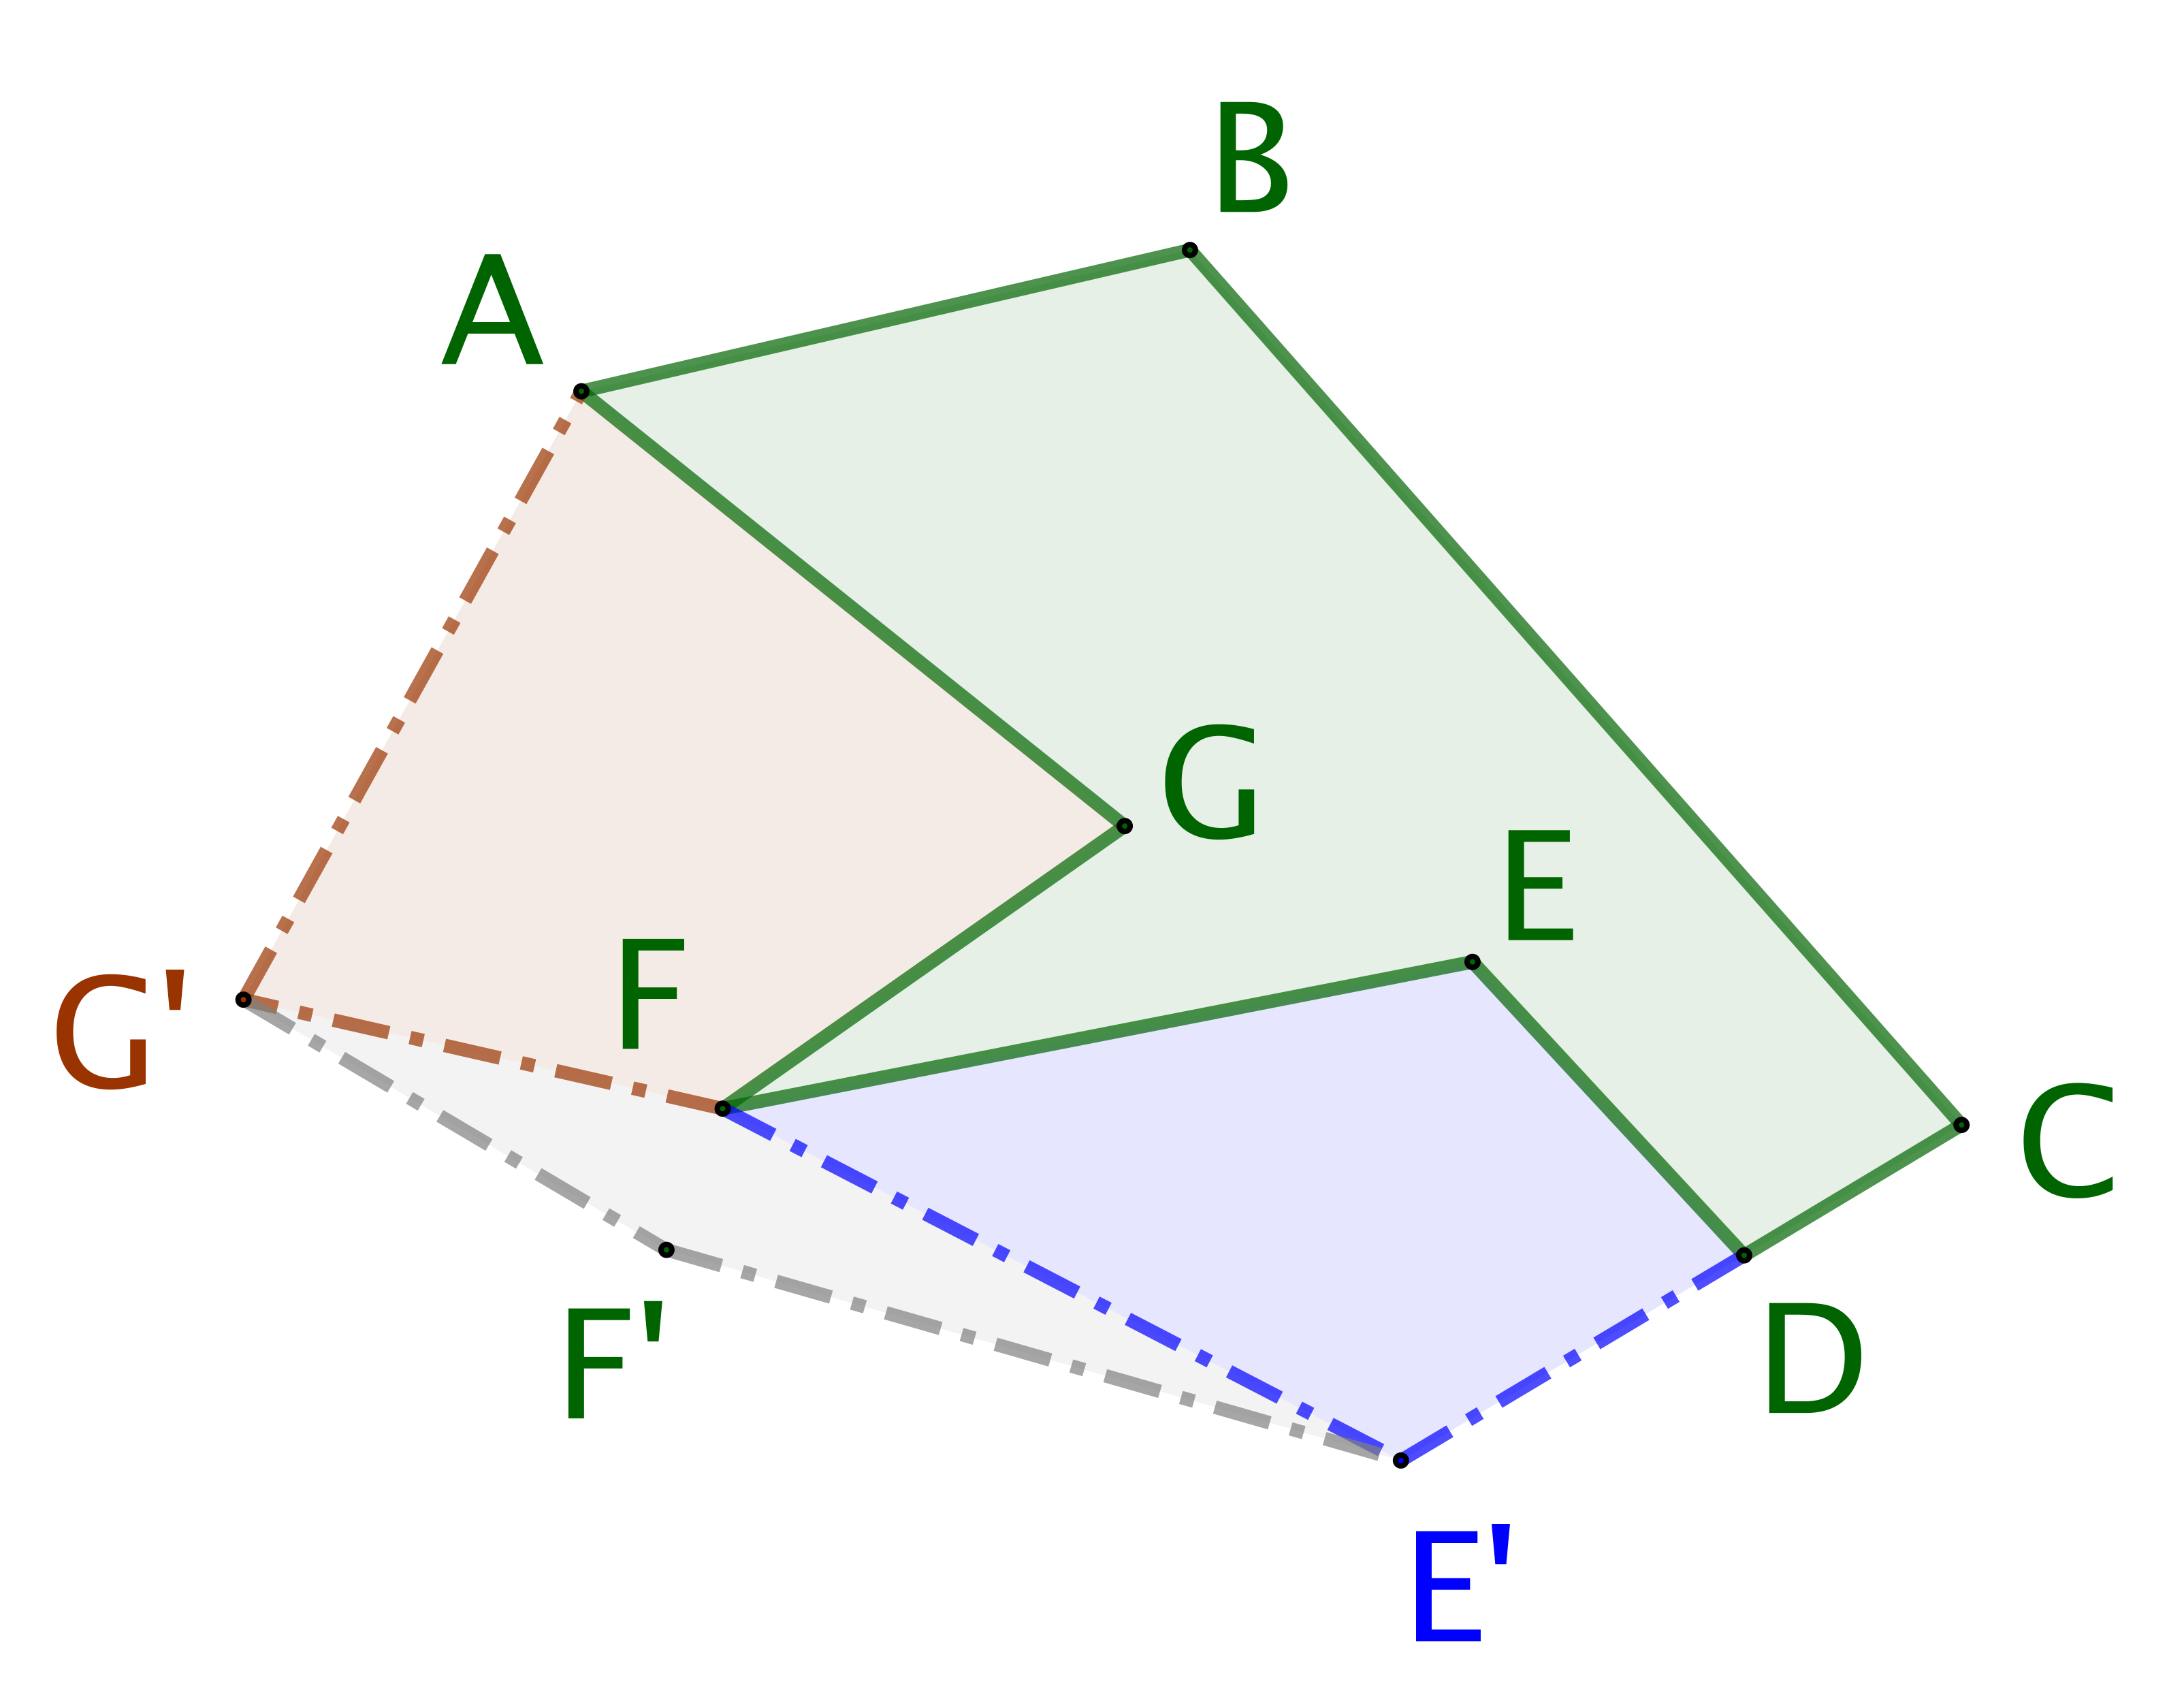
\includegraphics[scale=.4]{content/polygon/polygon-non-convex-bad.png}
	\end{center}


	Laissons de côté la construction précédente pour nous concentrer sur la classique enveloppe convexe%
	\footnote{
		C'est le plus petit polygone convexe \og \emph{contenant} \fg\ le \ngone\ considéré, où \og \emph{petit} \fg\ est relatif à l'inclusion.
	}
	du \ngone\ de départ.
	Par exemple, l'ennéagone $ABCDEFGHI$ non convexe ci-dessous admet le pentagone $ABDEG$ pour enveloppe convexe: le périmètre diminue et l'aire augmente, strictement tous les deux, ce qui est utile, mais malheureusement le nombre de côtés a diminué.
	
	\begin{center}
		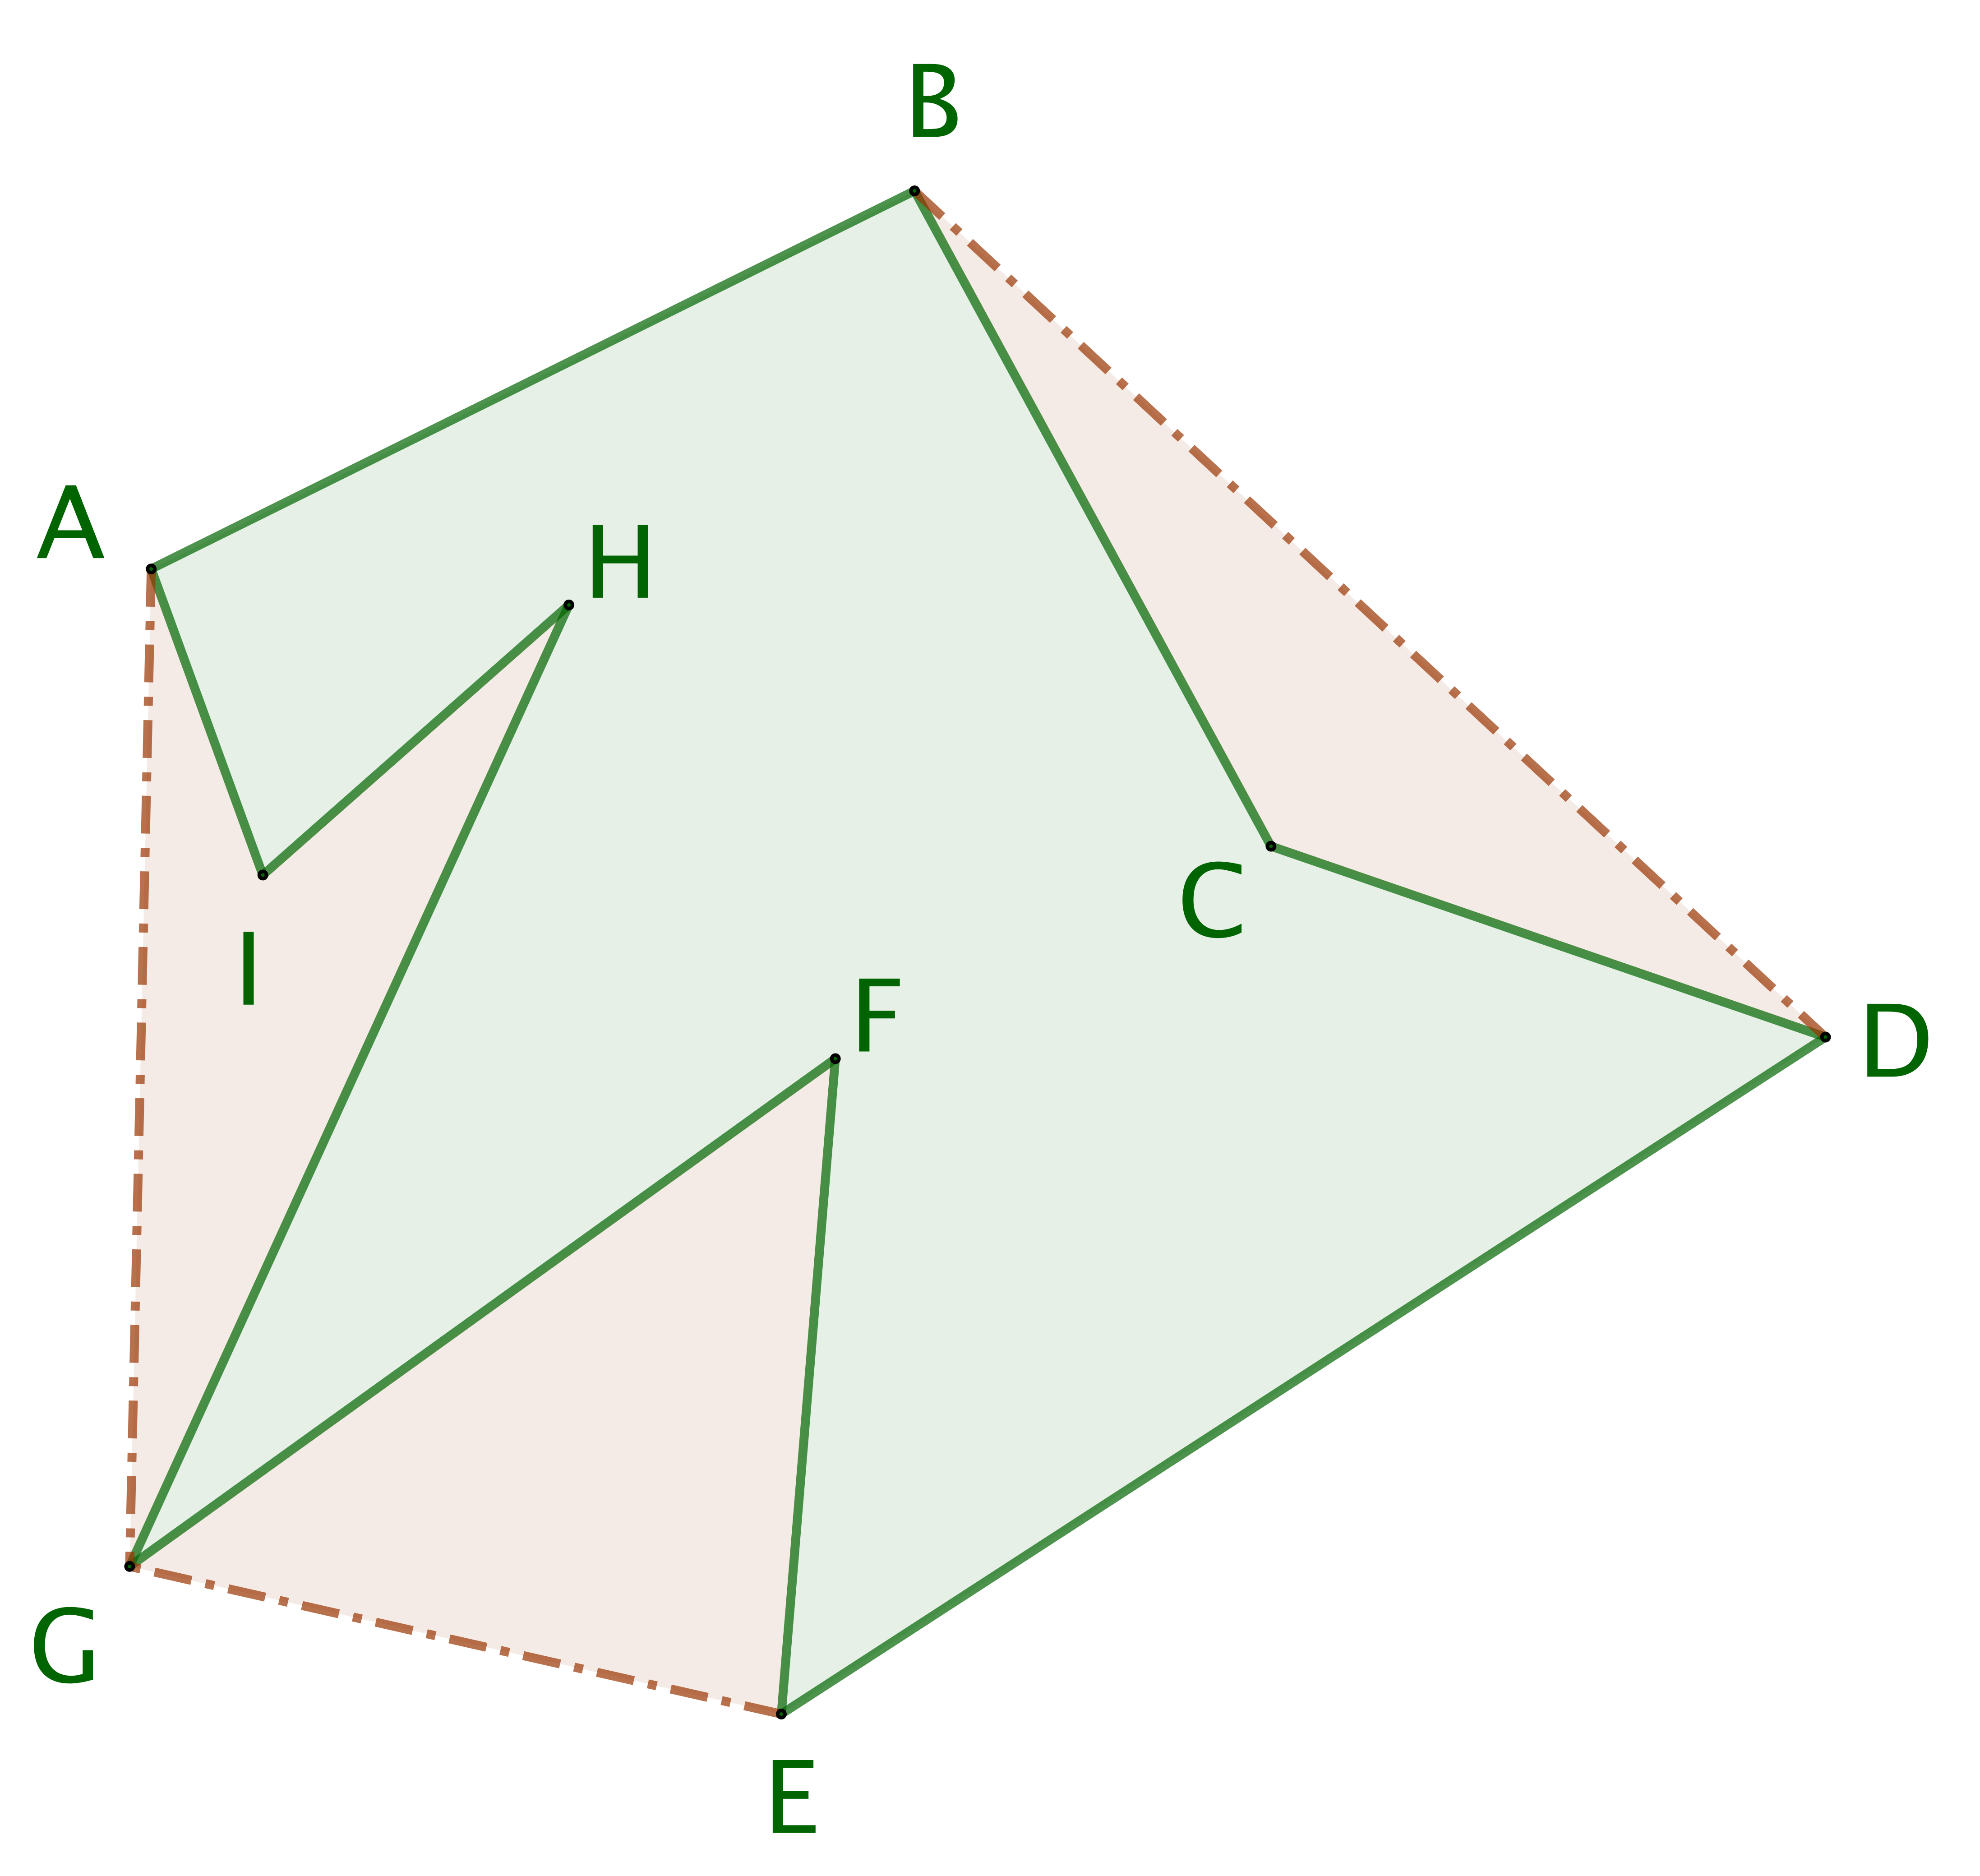
\includegraphics[scale=.4]{content/polygon/polygon-convex-hull.png}
	\end{center}

	Une idée simple, que nous allons formaliser rigoureusement après, consiste à ajouter les sommets manquants suffisamment prêts des côtés de l'enveloppe convexe pour ne pas perdre la convexité, tout en gardant un périmètre inférieur strictement au périmètre initial, et une aire strictement plus grande que l'aire initiale. Si nous arrivons à faire ceci, alors une homothétie de rapport $r > 1$ nous ramènera au bon périmètre avec une aire strictement plus grande que l'aire initiale.
	La figure suivante illustre cette idée.	
	
	\begin{center}
		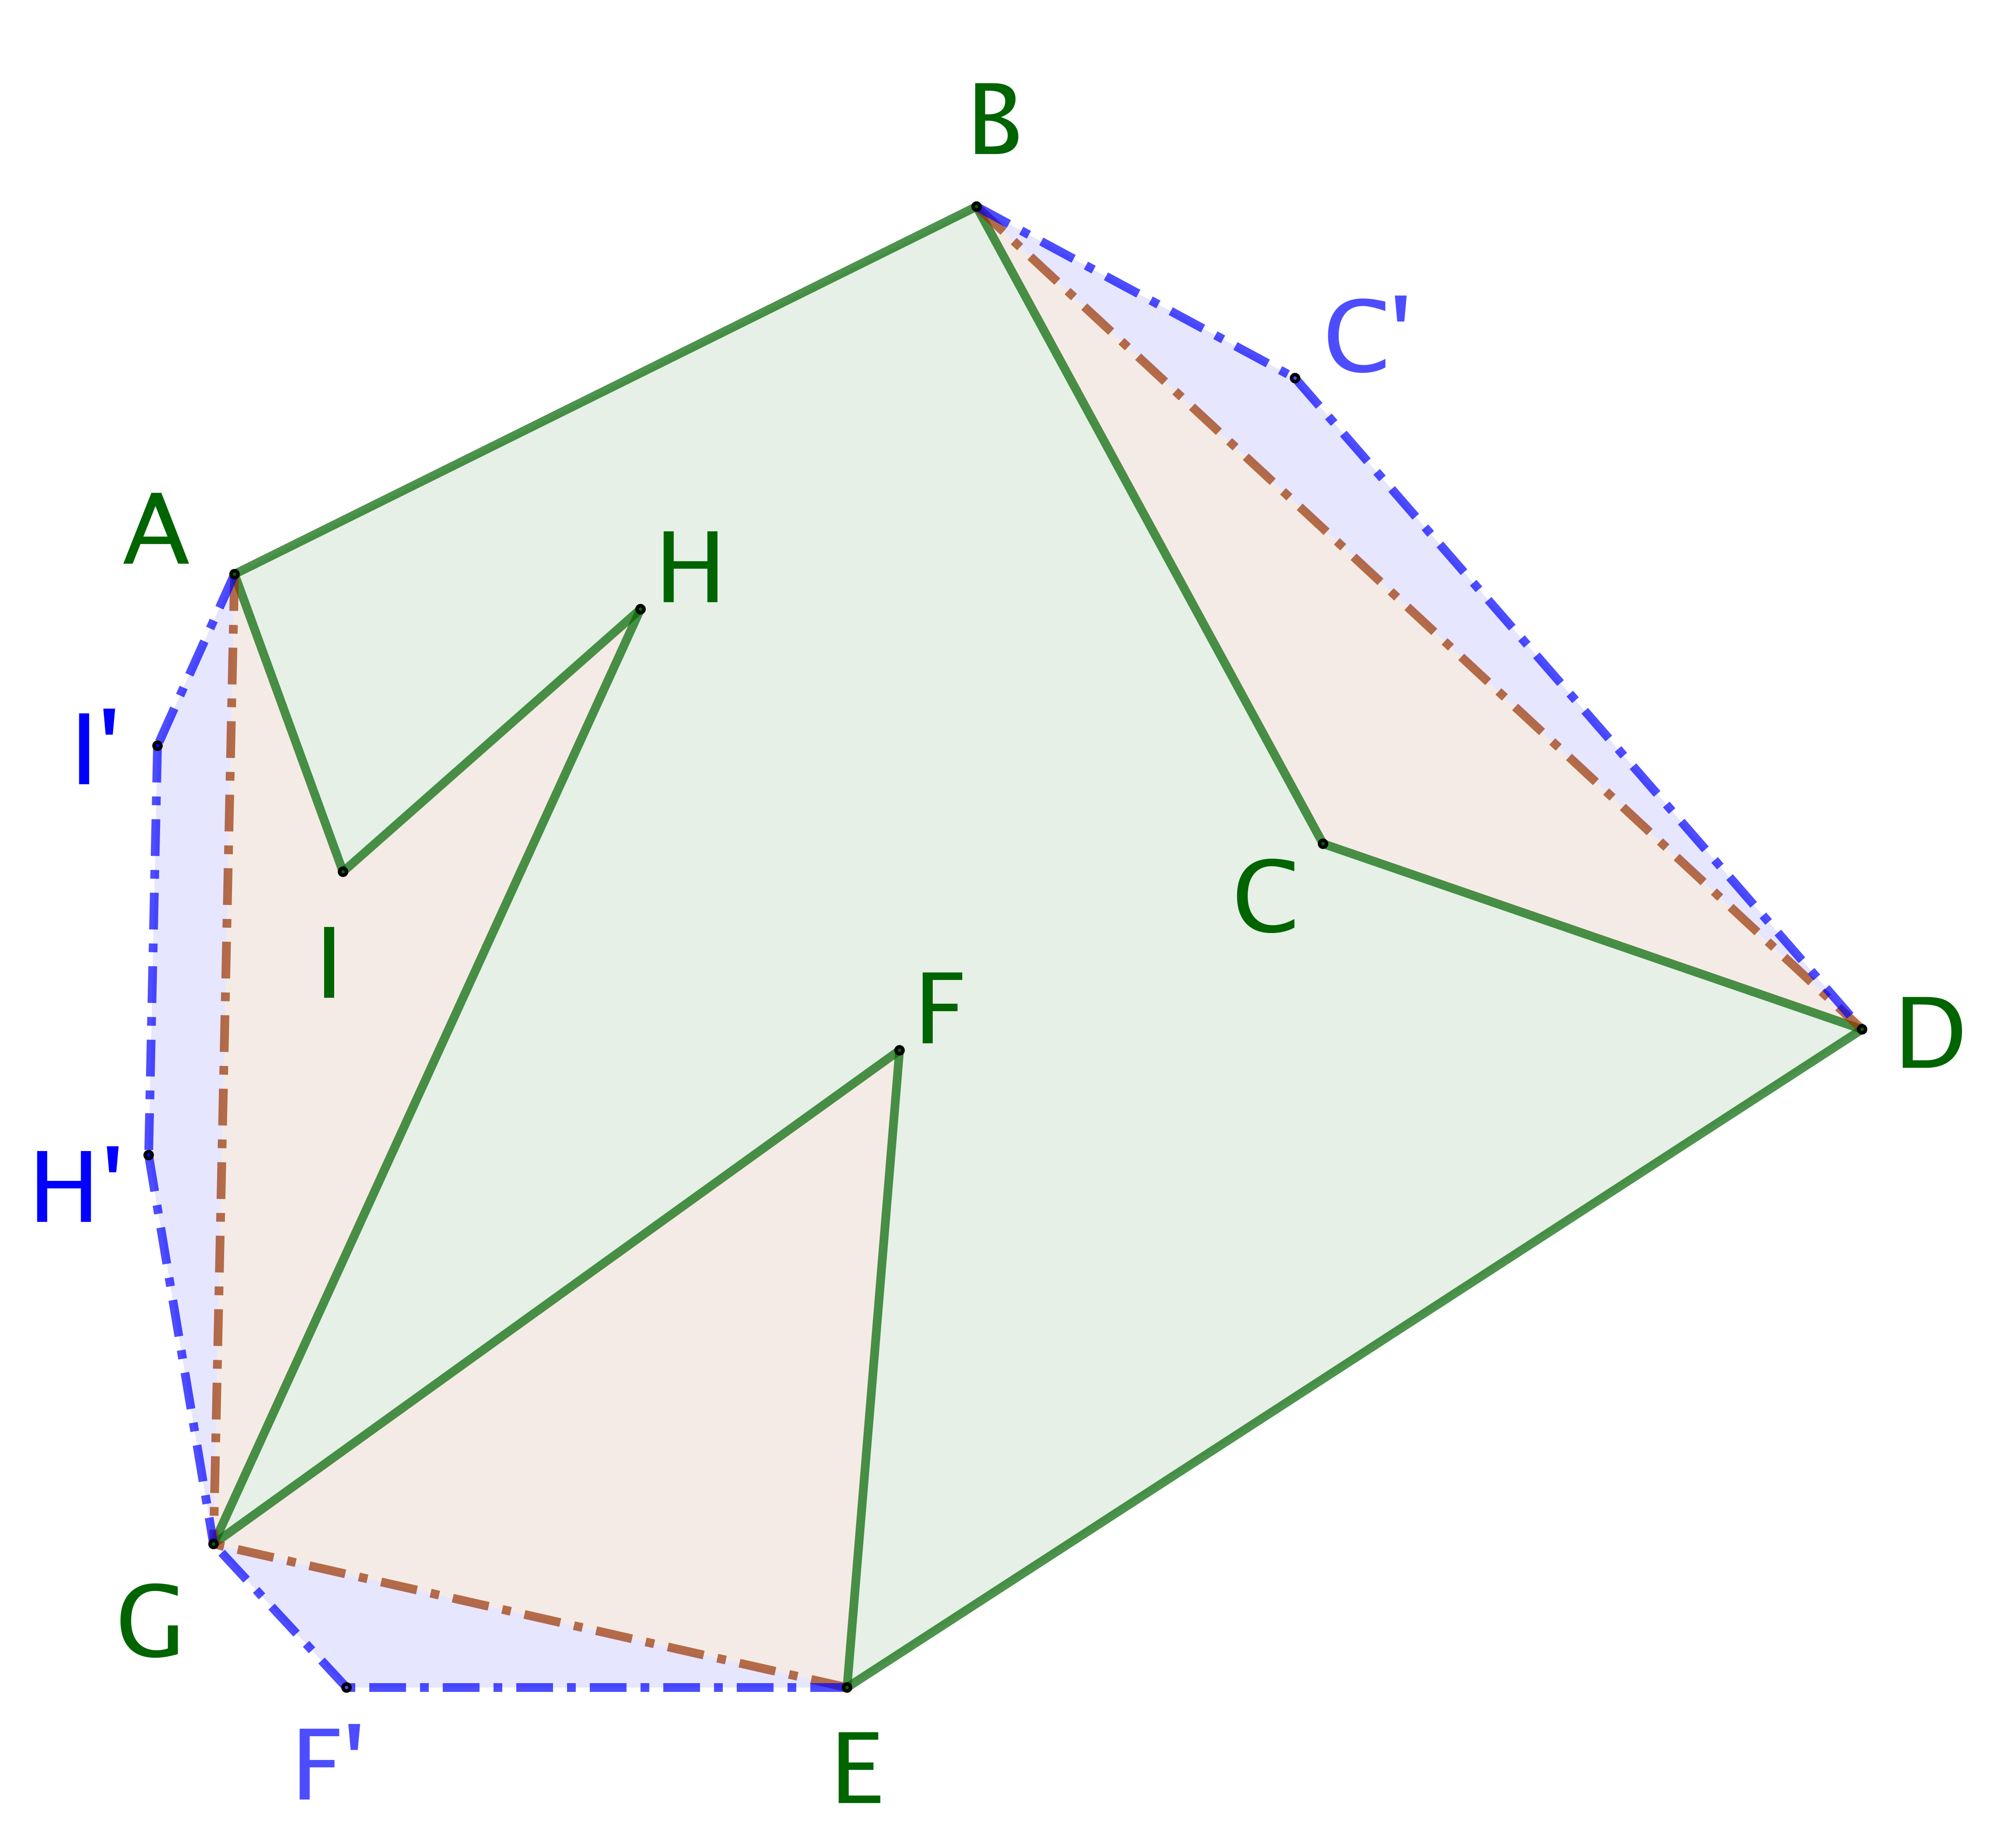
\includegraphics[scale=.4]{content/polygon/polygon-convex-hull-distortion.png}
	\end{center}

	Considérons donc un \ngone\ non convexe $\setproba{P}$, de périmètre $p$.
	%
	\begin{itemize}
		\item XXX

		\item XXX

		\item XXX

		\item XXX
	\end{itemize}
\end{proof}


\begin{remark}
	Le fait précédent permet de toujours se ramener au cas d'un \ngone\ convexe.
\end{remark}


% ----------------------- %


\begin{fact} \label{iso-poly} 
	Si un \ngone\ convexe $\setproba{P}$ n'est pas un \niso, alors on peut construire un \ngone\ convexe $\setproba{P}^{\,\prime}$ tel que 
	$\perim{\setproba{P}^{\,\prime}} = \perim{\setproba{P}}$ 
	et 
	$\area{\setproba{P}^{\,\prime}} > \area{\setproba{P}}$.
\end{fact}


\begin{proof}
	Considérons un \ngone\ convexe $\setproba{P}$ qui ne soit pas un \niso.
	Dans ce cas, $\setproba{P}$ admet un triplet de sommets consécutifs $A$, $B$ et $C$ tels que $AB \neq BC$ (sinon, on obtiendrait de proche en proche un \niso).
	La construction vue dans la preuve du fait \ref{tri-one-side-fixed} nous donne la solution: voir les deux dessins ci-après dans lesquels $(AC) \parallel (BB^{\,\prime})$. 
	Pour le 2\ieme\ cas, il n'est pas possible d'utiliser le triangle $AB^{\,\prime}C$ isocèle en $B^{\,\prime}$ car $(B^{\,\prime}C)$ porte le côté de sommet $C$ juste après $[BC]$, mais ce problème se contourne en considérant un point $B^{\,\prime\prime}$ de $]BB^{\,\prime}[$.
	%	
	\begin{multicols}{2}
		\centering

		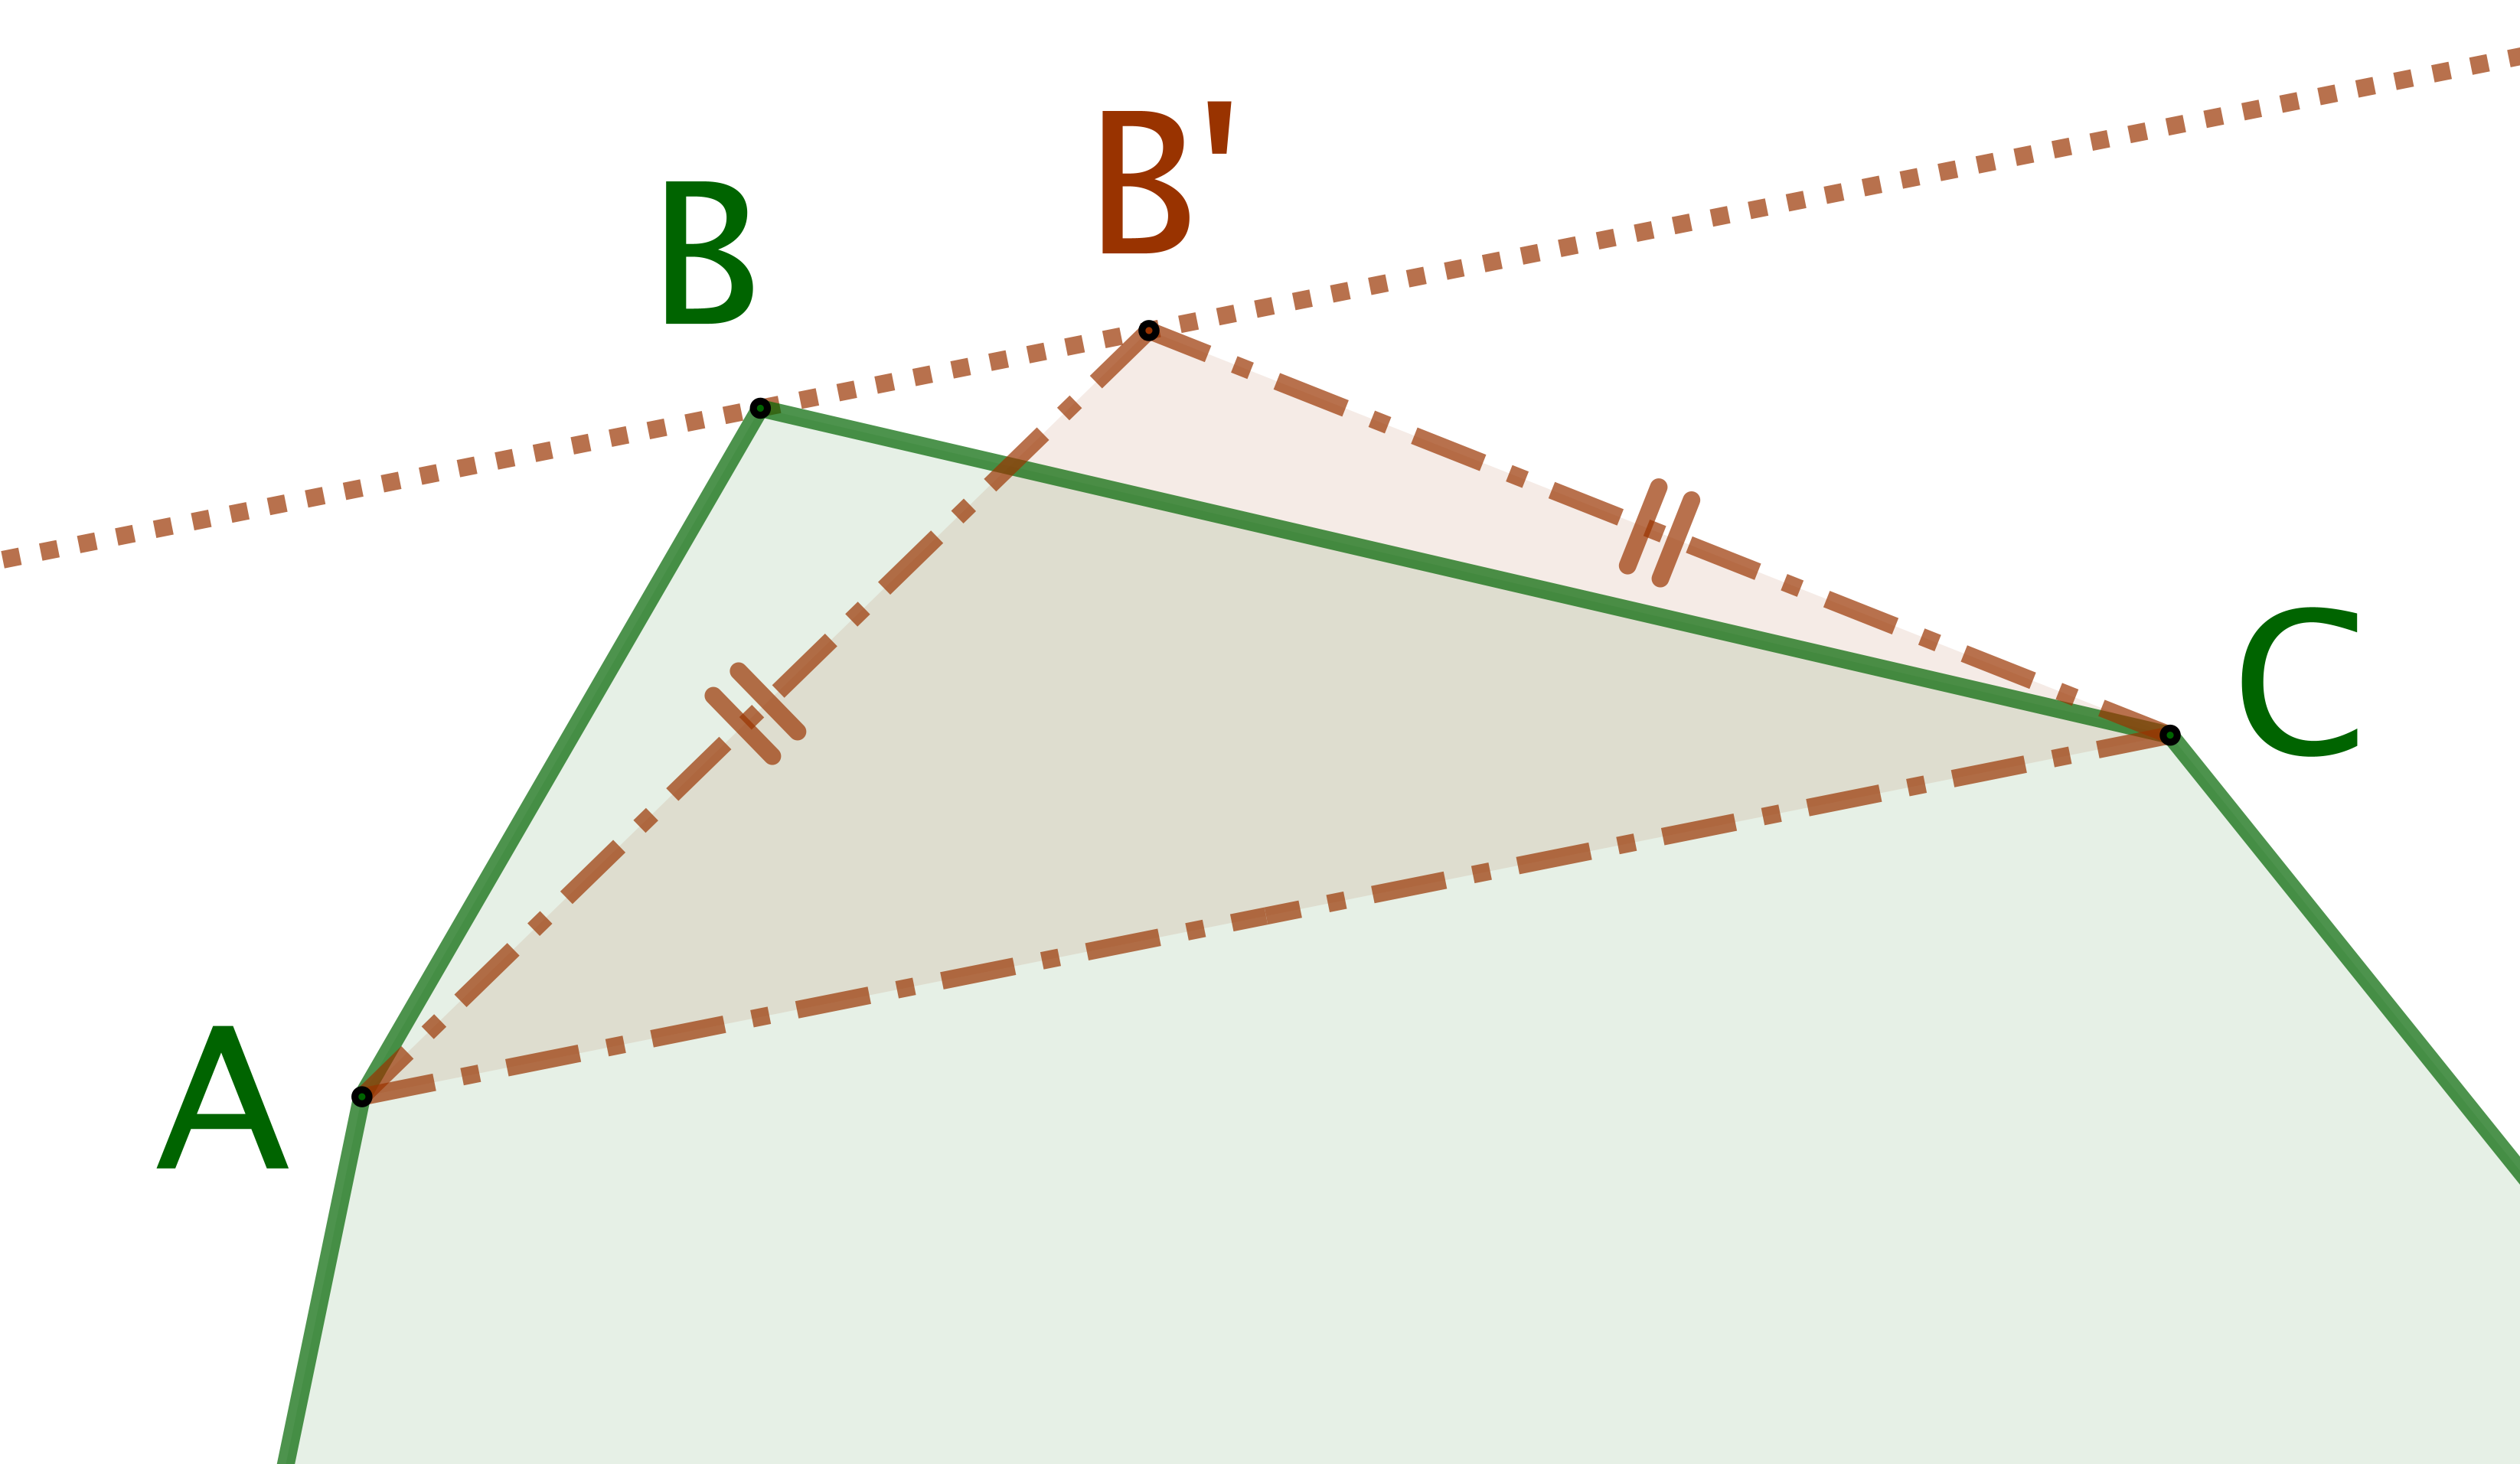
\includegraphics[scale=.4]{content/polygon/not-iso-OK.png}

		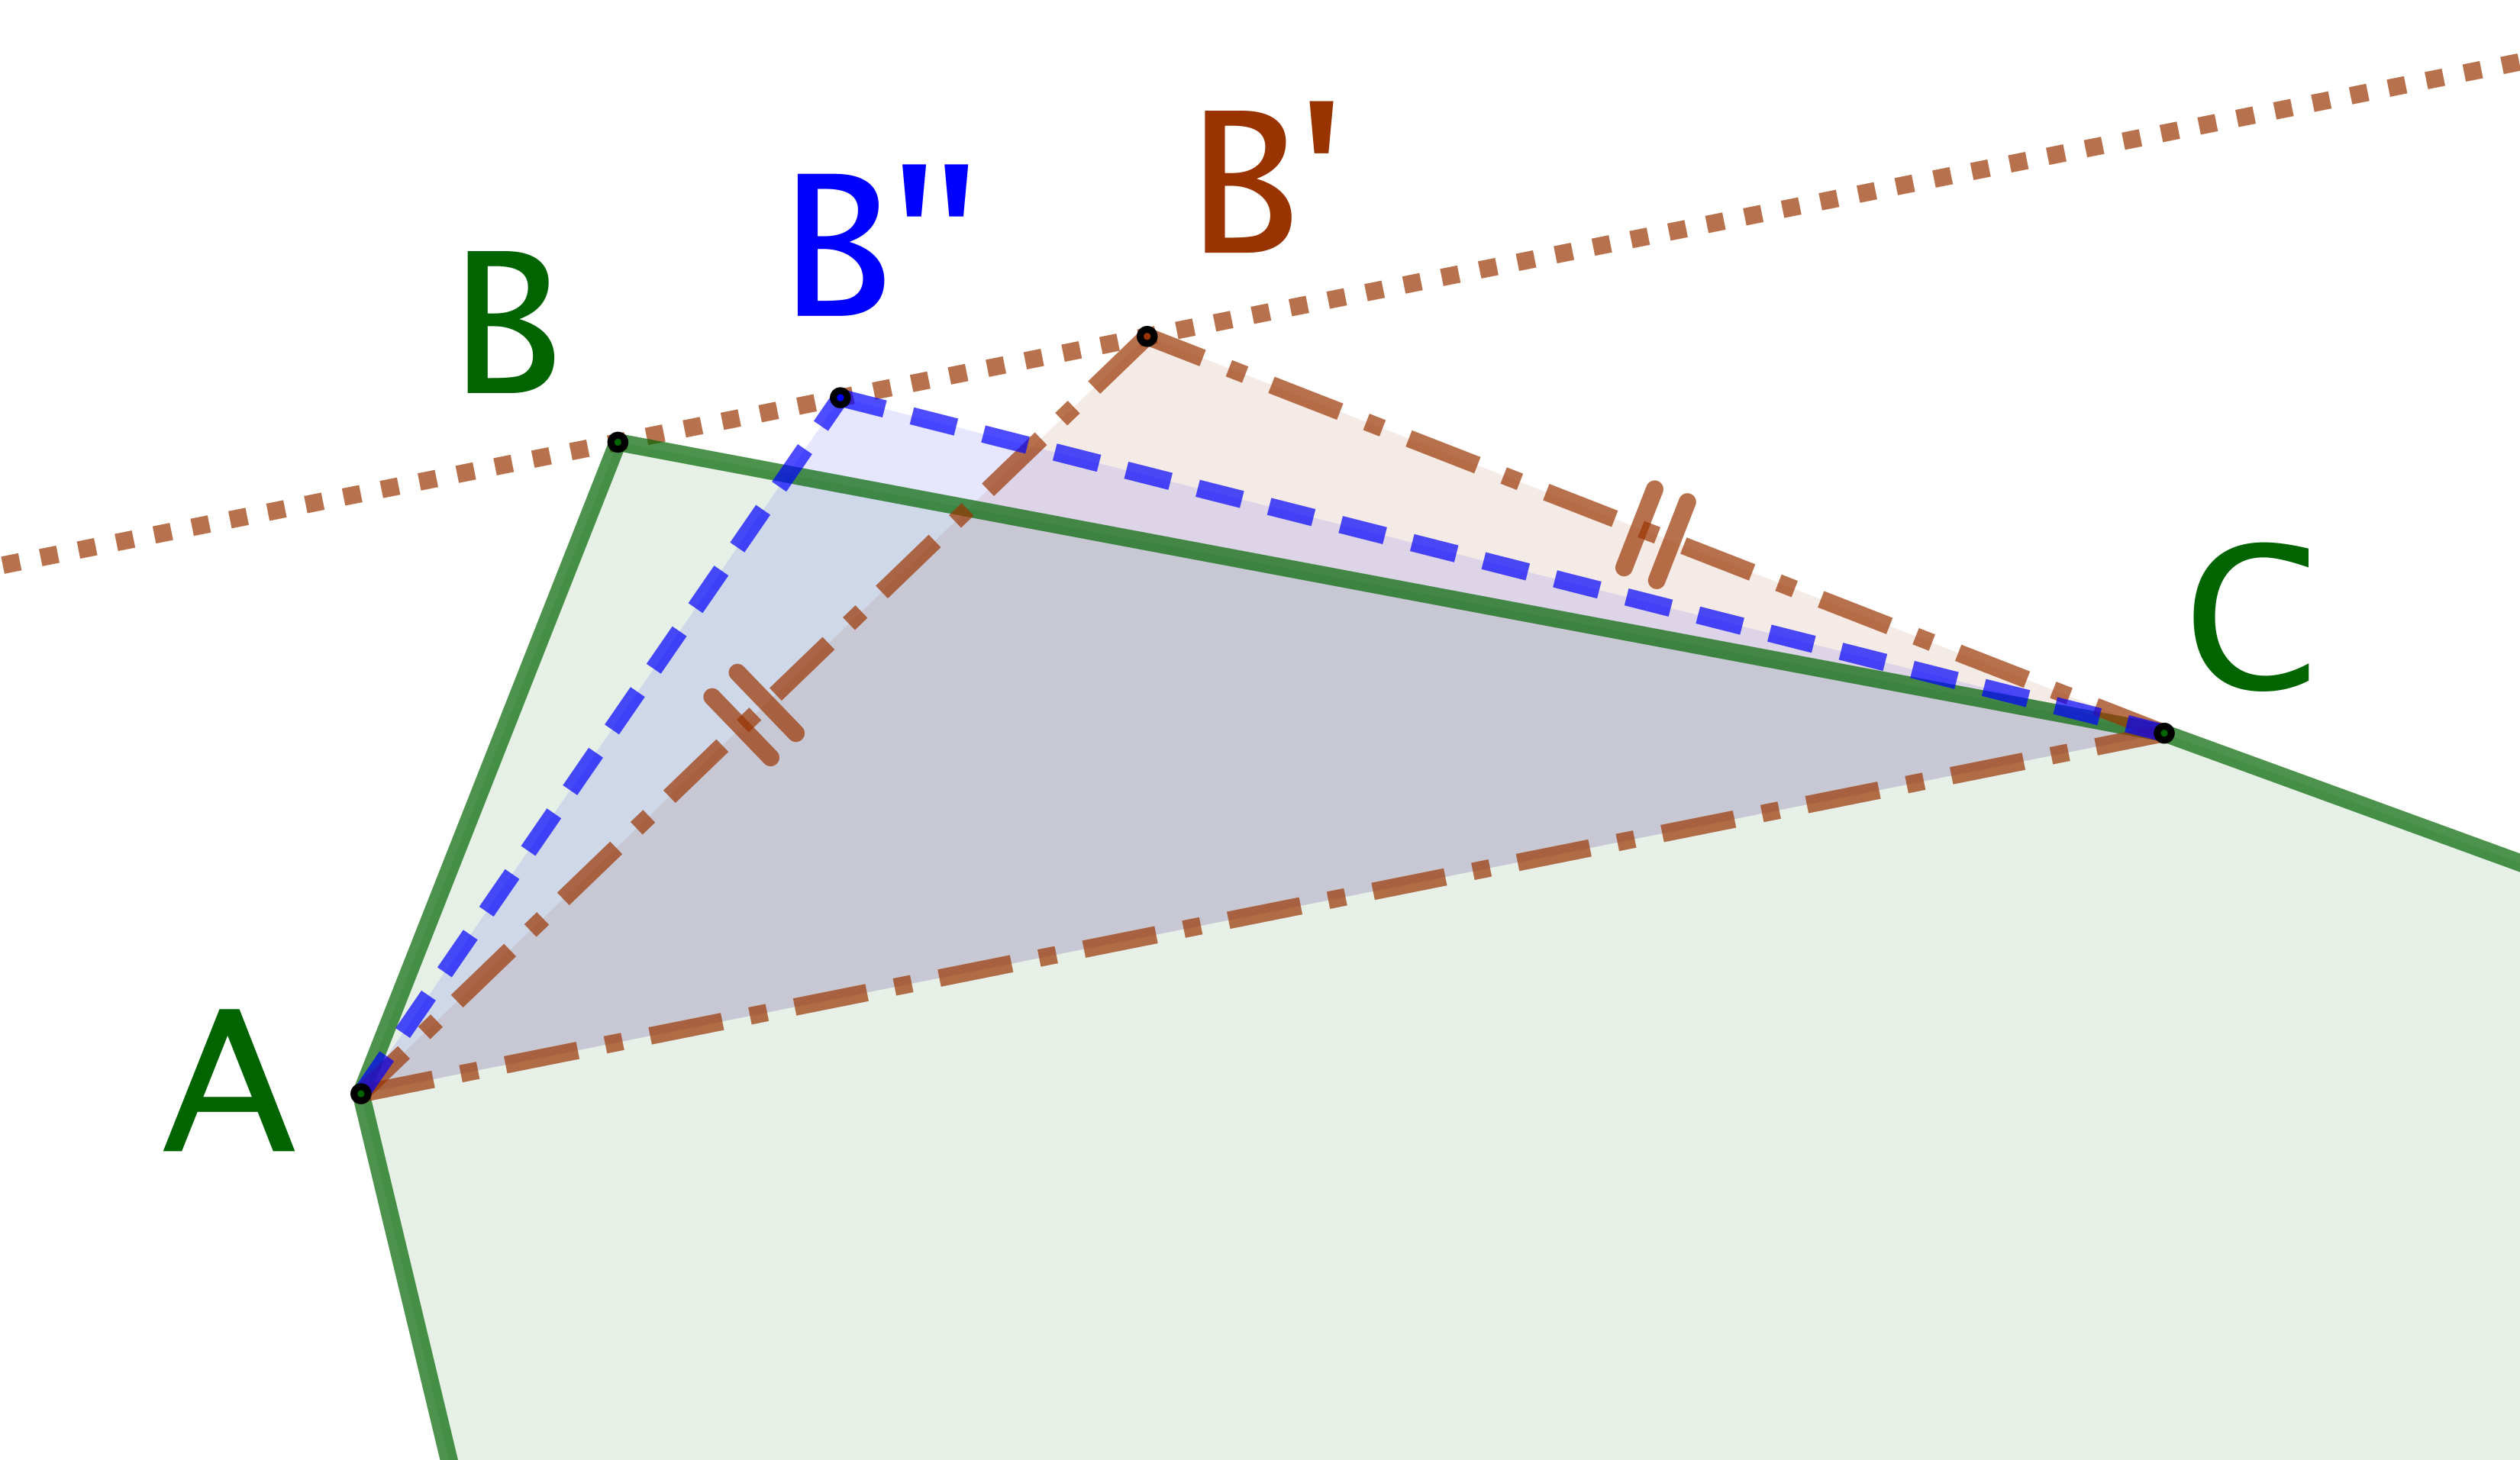
\includegraphics[scale=.4]{content/polygon/not-iso-KO.png}
	\end{multicols}
	
	Dans chaque cas, nous avons construit un \ngone\ convexe $\setproba{P}^{\,\prime\prime}$ tel que 
	$\perim{\setproba{P}^{\,\prime\prime}} < \perim{\setproba{P}}$ 
	et 
	$\area{\setproba{P}^{\,\prime\prime}} = \area{\setproba{P}}$.
	Un simple agrandissement donne un \ngone\ convexe $\setproba{P}^{\,\prime}$ vérifiant
	$\perim{\setproba{P}^{\,\prime}} = \perim{\setproba{P}}$ 
	et 
	$\area{\setproba{P}^{\,\prime}} > \area{\setproba{P}}$.
\end{proof}


\begin{remark}
	Le fait précédent ne permet pas de toujours se ramener au cas d'un \niso\ convexe. Il nous dit juste que si un \ngone\ convexe maximise son aire à périmètre fixé, alors il devra être un \niso. La nuance est importante, et nous pouvons en faire une similaire pour le fait suivant.
\end{remark}


% ----------------------- %


\begin{fact} \label{almost-reg-poly}
	Si un \niso\  convexe $\setproba{P}$ possède deux angles de mesures différentes,
	alors il existe un \ngone\ $\setproba{P}^{\,\prime}$ tel que
	$\perim{\setproba{P}^{\,\prime}} = \perim{\setproba{P}}$ 
	et 
	$\area{\setproba{P}^{\,\prime}} > \area{\setproba{P}}$.
\end{fact}


\begin{proof}
	wikipédia ok ? tjrs le pb du côté qui disparait !
	%
	\begin{itemize}
		\item XXX

		\item XXX

		\item XXX

		\item XXX
	\end{itemize}
\end{proof}


% ----------------------- %


\begin{fact}
	Soit $n \in \NN_{\geq3}$ un naturel fixé.
	Considérons tous les \ngones\  de périmètre fixé. Parmi tous ces \ngones, un seul est d'aire maximale, c'est le \ngone\ régulier.
\end{fact}


\begin{proof}
	Le fait \ref{conv-poly} permet de considérer le problème de maximisation d'aire à périmètre fixé uniquement avec des \ngones\ convexes.
	Selon les faits \ref{iso-poly} et \ref{almost-reg-poly}, si parmi les \ngones\ convexes de périmètre fixé, il en existe un qui maximise l'aire, alors ce ne peut être que le \ngone\ régulier.
	Pour voir que cette condition nécessaire est suffisante, comme dans le cas du triangle, voir la remarque \ref{tri-topo-comp}, nous convions le couple continuité/compacité comme suit.
	%	
	\begin{itemize}
		\item On munit le plan d'un repère orthonormé $\pvaxes{O | i | j}$. 

		\item 
		XXX
		
		fermeture costaud, mais le côté birné !!!!
		
		pour fermeture, besoin d'accpeter les \kgones\ pour $k \in \ZintervalC{3}{n}$.
		
		Les \ngones\ convexes $A_1 A_2 \cdots A_n$ tels que $\perim{A_1 A_2 \cdots A_n} = p$ sont représentés en posant $A_1\coord{0 | 0}$, $A_2\coord{A_1 A_2 | 0}$, puis $A_k\coord{x_k | y_k}$ avec $y_k \geq 0$ pour $k \in \ZintervalC{3}{n}$. Un \ngone\ peut donc avoir $n$ représentations, mais peu importe.
		De plus, on accepte les \ngones\ dégénérés pour lesquels nous avons $x_B = 0$, $y_C = 0$ dans notre représentation.
		Nous notons alors $\setproba{G} \subset \RR^{2n}$ l'ensemble des triplets $\coord{x_B | x_C | y_C}$ ainsi obtenus.

		\item XXX
		
		Justifier que $\setproba{G}$ est fermé dans $\RR^{2n}$.

		\item $\setproba{G}$ est aussi borné, car les coordonnées des sommets des \ngones\ convexes considérés le sont.		
		En résumé, $\setproba{G}$ est un compact de $\RR^{2n}$.

		\item Notons $s: \setproba{G} \rightarrow \RRp$ la fonction \og \emph{aire} \fg\ des \ngones\ représentés. 
		Cette fonction est continue en les coordonnées des sommets, car elle peut être calculée comme suit pour un \ngone\ convexe $A_1 A_2 \cdots A_n$ quelconque.
		%
		\begin{enumerate}
			\item L'isobarycentre $G$ de $A_1 A_2 \cdots A_n$ possède des coordonnées affines en celles des points $A_1$, $A_2$, \dots\ , et $A_n$.

			\item Par convexité, l'aire de $A_1 A_2 \cdots A_n$ est égale à la somme de celles des triangles $G A_k A_{k+1}$ pour $k \in \ZintervalC{1}{n-1}$, et du triangle $G A_n  A_1$.

			\item Via le déterminant, il est immédiat de voir que les aires des triangles considérés sont des fonctions continues en les coordonnées des sommets.
		\end{enumerate}
		
		
		\item Finalement, par continuité et compacité, on sait que $s$ admet un maximum sur $\setproba{G}$. 
		Chapeau bas à vous, Géométrie et Analyse réunies...
	\end{itemize}	
\end{proof}
